% =========================================================================== %
\chapter{Архитектура программной реализация}\label{chap3_soft_architecture}
% =========================================================================== %
Была проведена реорганизация исходного кода программного каркаса, в результате которой было выделено 3 модуля. Текущая структура каталогов проекта представлена на рисунке~\ref{fig:fileStructure}.
\begin{figure}[!ht]
    \centering
    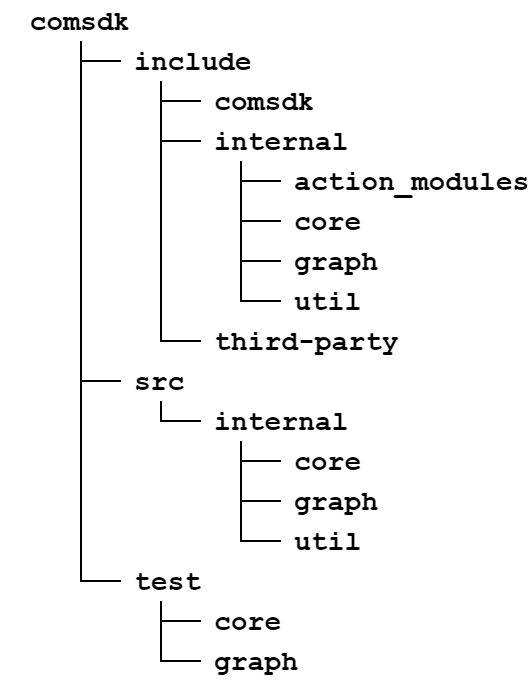
\includegraphics[height=0.35\textheight]{figures/fileStructure.png}
    \caption{Структура каталогов проекта}
    \label{fig:fileStructure}
\end{figure}
Были выделены отдельные каталоги для заголовочных файлов, где объявлены интерфейсы разработанных структур данных, и для файлов с их реализациями (\textsf{include/internal} и \textsf{src/internal} соответственно). Кроме того, создан отдельный каталог для публичных заголовочных файлов библиотеки \textsf{include/comsdk}, которые будут использоваться конечным пользователем при разработке программных реализаций различных алгоритмов.
% --------------------------------------------------------------------------- %
\section{Требования к алгоритму обхода графовых моделей}\label{sec:algorithm_task}
% --------------------------------------------------------------------------- %

Методология GBSE подразумевает параллельное независимых ветвей графа. На рисунке \ref{fig:parallelExample} после выполнения рёбер $F_{12}$~и~$F_{13}$ будет получено два независимых состояния данных $S_2$ и $S_3$ соответственно. Далее возникает задача правильным образом перевести данные из этих состояний в общее состояние $S_4$.
\begin{figure}[!ht]
    \centering
    \includegraphics[scale=0.4]{figures/example.parallel.png}
    \caption{Пример графовой модели, требующей параллельного исполнения}
    \label{fig:parallelExample}
\end{figure}

Данный подход значительно увеличивает эффективность использования ресурсов вычислительной системы и ускоряет процесс решения, однако добавляет некоторые второстепенные задачи при разработке. Так в примере на рисунке \ref{fig:parallelExample} рёбра $F_{12}$~и~$F_{13}$ выполнялись параллельно, а значит полученные в результате их выполнения данные существуют в самом общем случае в различных адресных пространствах оперативной памяти (возможно даже на двух разных вычислительных машинах). В момент разветвления графа должно происходить корректное предоставление вычислительным ресурсам (потокам, процессам, узлам кластера и т.п.) доступа к обрабатываемым данным. Помимо этого алгоритм обхода графовой модели должен корректно отрабатывать слияние ветвей графа и в частности при необходимости выполнять сбор данных.

\begin{figure}[!ht]
    \centering
    \includegraphics[scale=0.4]{figures/example.parallel_then_linear.png}
    \caption{Пример графовой модели с совмещением ветвей}
    \label{fig:parallelThenLinearExample}
\end{figure}

На рисунке \ref{fig:parallelThenLinearExample} ветви $S_1 \rightarrow S_2 \rightarrow S_4$ и $S_1 \rightarrow S_3 \rightarrow S_4$ выполняются с использованием различных вычислительных ресурсов, но ребро $F_{45}$ выполняется в пределах одной <<общей>> ветви графа $S_4 \rightarrow S_5$, и в момент его выполнения ресурсы, выделенные на выполнение двух паралельных ветвей уже не требуются. Таким образом, целесообразно разработать управляющую структуру, которая бы отвечала за выделение и освобождение вычислительных ресурсов во время работы с несколькими параллельными ветвями графа.

Кроме того, разрабатываемая архитектура должна поддерживать несколько вариантов параллельного исполнения. Среди прочих желательна поддержка:
\begin{itemize}
    \item поочерёдного выполнения (в первую очередь для отладки) в одном потоке управления;
    \item выполнения с использованием нескольких процессов операционной системы;
    \item выполнения с использованием нескольких потоков процессора;
    \item выполнения на удалённых узлах (через SSH-соединение).
\end{itemize}

Таким образом целесообразна поддержка единого интерфейса обозначенной управляющей структуры для разных режимов выполнения (последовательный, параллельный, распределённый и пр.).

В случае, когда параллельного выполнения не требуется и предусмотрено условное ветвление, оно должно быть реализовано при помощи специальных функций, привязываемых к узлам графовой модели. В контексте <<графоориентированного подхода>> такие функции называются \emph{селекторами}. Формально функция-селектор $h_i$, привязанная к узлу $v_i$, должна входному набору данных $\bar{D}$ ставить в соответствие множество рёбер $E_i$, выходящих из $v_i$, проход по которым нужно совершить. Пример работы функции-селектора демонстрирует рисунок~\ref{fig:graphSelector}.

\begin{figure}[H]
    \centering
    \includegraphics[width=\textwidth]{figures/example.selector.png}
    \caption{Пример фрагмента графовой модели с функцией-селектором}
    \label{fig:graphSelector}
\end{figure}

На рисунке~\ref{fig:graphSelector} красным обозначено ребро, переход по которому будет совершён после вызова функции-селектора.

Алгоритмы обхода графовых моделей, предусматривающие условное ветвление и параллельное выполнение ветвей представлены в разделе~\ref{sec:algorithm_task}.
% --------------------------------------------------------------------------- %
\section{Функциональные структуры данных}\label{sec:functional_classes}
% --------------------------------------------------------------------------- %
Поскольку методология GBSE позволяет во время работы алгоритма загружать функции-предикаты, функции-обработчики и функции-селекторы из стандартных или пользовательских динамических библиотек, требовалась некоторая абстракция вида <<функция, загружаемая из динамической библиотеки>>. При анализе исходных компонентов библиотеки comsdk, было обнаружено, что такая абстракция уже реализована в классе \textsf{ActionItem}. Он представляет собой абстракцию над любой функциональной возможностью реализуемой системы. Изначально входными данными для такой абстракции мог быть только объект класса \textsf{Anymap}, поэтому был разработан шаблон класса для поддержки различных типов входных данных. UML-диаграмма разработанных шаблонов классов предствлена на рисунке~\ref{fig:UMLActionItems}.
\begin{figure}[!ht]
    \centering
    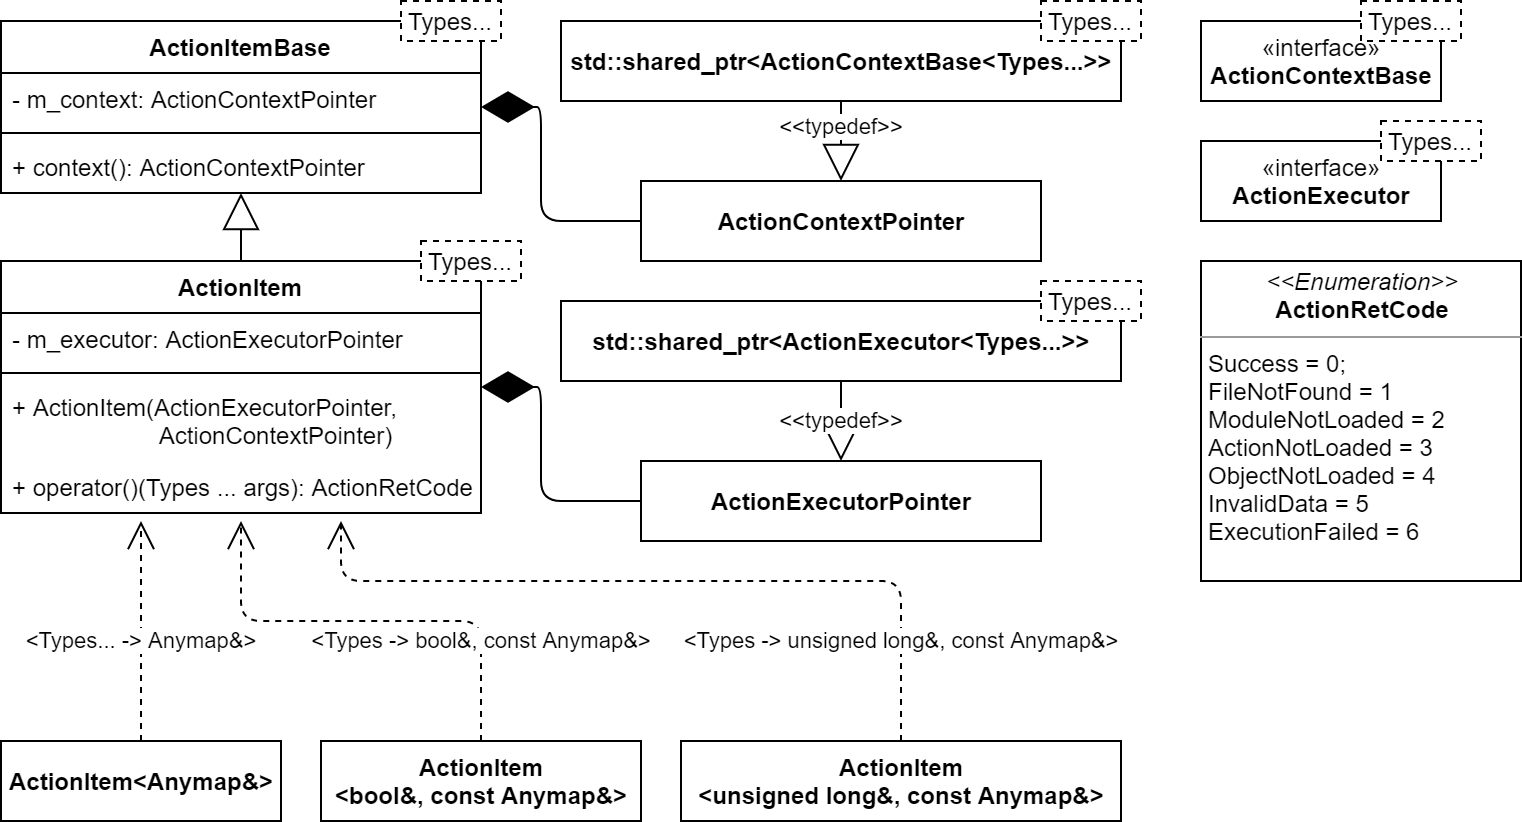
\includegraphics[width=0.95\textwidth]{figures/UML.actionItem.png}
    \caption{Структура классов, описывающих функциональные возможности системы}
    \label{fig:UMLActionItems}
\end{figure}
Запуск функциональной возможность осуществляется посредством перегруженного оператора вызова. Для реализации обработчиков, предикатов и селекторов были созданы специализации шаблона \textsf{ActionItem}, которые были использованы в качестве базовых классов.

% --------------------------------------------------------------------------- %
\section{Информационные структуры данных}
% --------------------------------------------------------------------------- %
\begin{figure}[!ht]
    \centering
    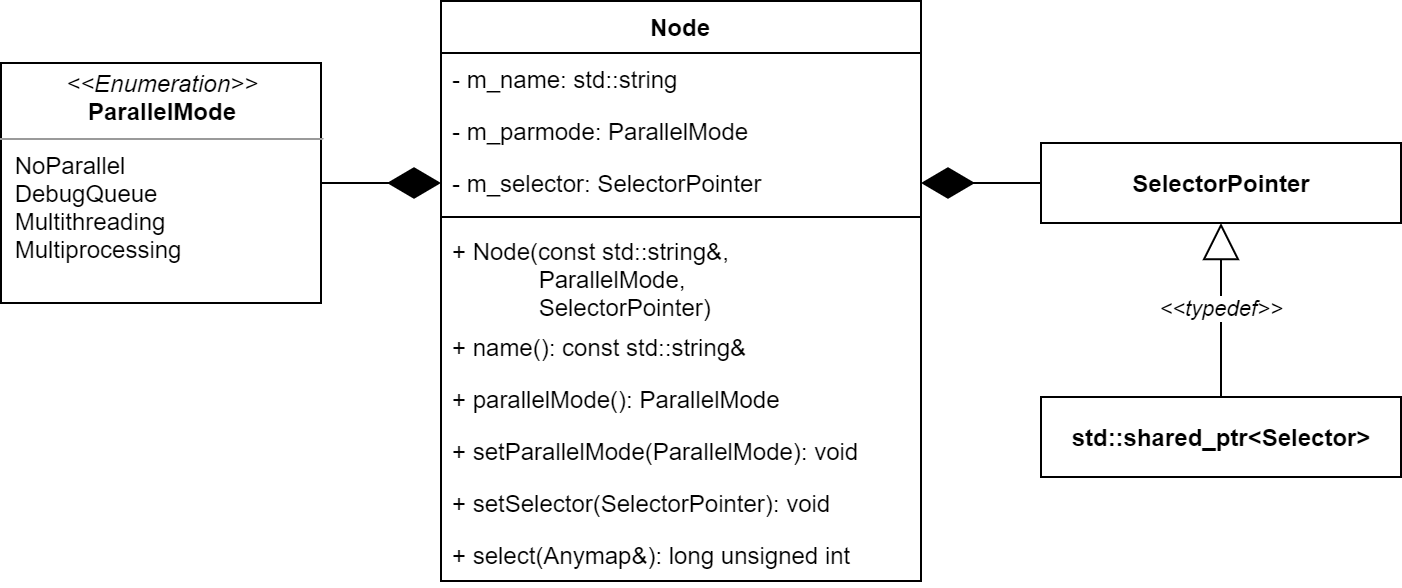
\includegraphics[height=0.25\textheight]{figures/class.node_v2.png}
    \caption{UML-описание вершины графовой модели}
    \label{fig.UMLNode}
\end{figure}
Структура данных, описывающая вершину графовой модели, хранит в себе имя вершины, режим параллельного обхода нескольких ветвей, выходящих из данной вершины и указатель на функцию-селектор, реализация которых описана в разделе~\ref{sec:functional_classes}.
% --------------------------------------------------------------------------- %
\section{Управляющие структуры данных}
% --------------------------------------------------------------------------- %
Основной структурой данных, поддерживающей разработанный алгоритм обхода (описан в разделе~\ref{sec:algorithm_desc}) является структура данных <<контейнер выполнения>>. Задача её внутренней логики -- контролировать параллельный обход нескольких ветвей графа и отслеживать их слияние. Помимо прочего это подразумевает выделение и освобождение вычислительных ресурсов для параллельного обхода. Поскольку в общем случае могут применяться различные вычислительные ресурсы (потоки ядер процессора, процессы операционной системы, узлы вычислительного кластера и пр.), было принято решение разработать единый интерфейс структуры <<контейнер выполнения>> без привязки к конкретным ресурсам. Это позволит независимо разрабатывать различные реализации данной структуры для различных режимов параллельного обхода.

Помимо прочего при проектировании интерфейса структуры данных <<контейнер выполнения>> были задействованы разработанные информационные структуры данных <<операция с вершиной>> (\textsf{NodeOp}) и <<операция с ребром>> (\textsf{EdgeOp}).

Интерфейсы спроектированных структур данных были описаны с помощью UML-диаграмм, представленных на рисунке \ref{fig:UMLAll}. Были учтены особенности описания классов на языке C++.

\begin{figure}[!ht]
    \centering
    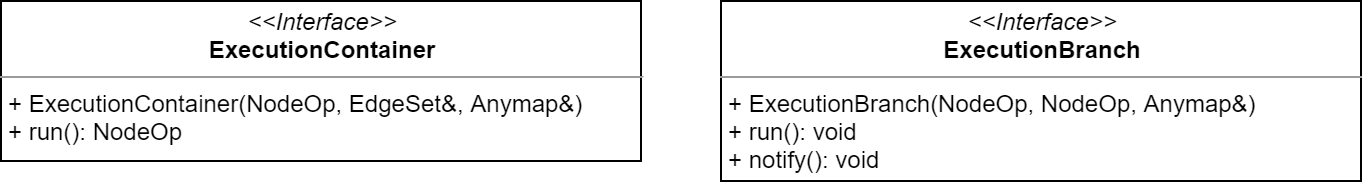
\includegraphics[width=\textwidth]{figures/UML.all.png}
    \caption{UML-диаграммы разработанных структур данных}
    \label{fig:UMLAll}
\end{figure}

Конструктор класса \textsf{ExecutionContainer} соответствует алгоритму, описанному в разделе~\ref{sec:algorithm_desc}. Метод run выполняет алгоритм, описанный блок-схемой на рисунке~\ref{fig:flowchartExecutionContainer}.

Кроме того, была спроектирован интерфейс структуры <<ветви исполнения>> (\textsf{ExecutionBranch} на рисунке~\ref{fig:UMLAll}). Её задача -- выполнение обхода одной конкретно взятой ветви (метод \textsf{run()}) графовой модели с уведомлением <<контейнера исполнения>> о завершении каждой функции перехода (метод \textsf{notify()}), как того требует алгоритм.

Таким образом, разработанные классы реализуют в себе логику параллельного обхода ветвей графовой модели и хранят данные в соответствии с разработанной процедурой обхода.

